
The given equation can be expressed as 
\begin{align}
\vec{x}^T \myvec{2 & 0\\0 & 0}\vec{x}+ \myvec{-4 & 0}\vec{x}+3=0
\end{align}
%
The discriminant is 
\begin{align}
D &= b^2 - 4ac
\\
&=-8 \quad < 0
\end{align}
Thus  the equation has no real roots as can be seen from Fig. \ref{quadform/24/Roots of $2x^2 -4x + 3 = 0$}.
%
\begin{figure}[!ht]
\centering
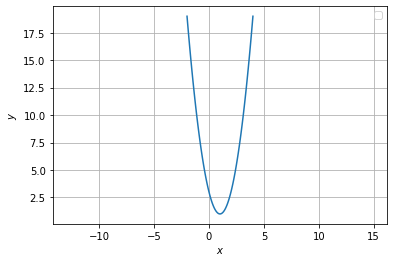
\includegraphics[width=\columnwidth]{solutions/su2021/2/24/diagram.png}
\caption{Roots of $2x^2 -4x + 3 = 0$ }
\label{quadform/24/Roots of $2x^2 -4x + 3 = 0$}
\end{figure}


